% 原文PDF278--304：第8.5--8.8節および第8章の全演習。
\subsectionlink{オービフォールド}\label{sec:8.5}

$X^{25}$ を周期的に同一視する代わりに、反射
\begin{equation}
X^{25}\cong-X^{25}
\tag{8.5.1}\label{eq:8.5.1}
\end{equation}
によって点を同一視することを考えよう。この場合、基本領域は半直線 $X^{25}\geq0$ であり、超平面 $X^{25}=0$ が境界となる。この超平面は、その各点が反射 (8.5.1) によって不動であるという点で特別である。より一般には、$k$ 個の座標を同時に反射する変換
\begin{equation}
X^m\longrightarrow-X^m,\qquad 26-k\leq m\leq25
\tag{8.5.2}\label{eq:8.5.2}
\end{equation}
によって時空を同一視できる。この場合にも、$X^{26-k}=\cdots=X^{25}=0$ に固定点の空間がある。$k\geq2$ では、この空間は特異点となる。特に $k=2$ では、欠損角 $\pi$ の円錐特異点である。

反射 (8.5.1) と周期的な同一視 $X^{25}\cong X^{25}+2\pi R$ を組み合わせると、コンパクト空間を作れる。これらをそれぞれ $r$ と $t$ と呼ぼう。まず $t$ によって同一視して円 $S^1$ を作り、次に円上の点を $r$ によって同一視すると考えてよい。得られるコンパクト空間は線分で、$0\leq X^{25}\leq\pi R$ を基本領域とする。線分の両端には固定点があり、点 $\pi R$ は $tr$ によって不動である。全体として、任意の整数 $m$ に対して、群
\begin{align}
t^m:\quad&X^{25}\cong X^{25}+2\pi Rm,
\tag{8.5.3a}\label{eq:8.5.3a}\\
t^mr:\quad&X^{25}\cong2\pi Rm-X^{25}
\tag{8.5.3b}\label{eq:8.5.3b}
\end{align}
の作用で実直線を同一視している。

同様に、$k$ 次元トーラスを反射 (8.5.2) によって同一視してもよい。この場合、互いに異なる固定点が $2^k$ 個あり、各 $X^m$ は $0$ または $\pi R$ である。このようにして得られる特異な空間を\textbf{オービフォールド}という。非コンパクト空間を (8.5.2) によって同一視して得られる空間は $\mathbb R^k/\mathbb Z_2$ であり、$k$ 次元トーラスに同じ同一視を施して得られるコンパクト空間は $T^k/\mathbb Z_2$ である。

このような特異空間上の弦理論が意味をもつことは自明ではないが、実際に意味をもつことがわかる。これはトーラスコンパクト化とそれほど異ならないものの、より多くの対称性を、後には超対称性も破るので、弦模型の構成にとって興味深い。

同一視 (8.5.1) または (8.5.2) には二つの効果がある。第一に、弦の波動関数は反射に対して不変、すなわち同一視された点で等しくなければならない。第二に、閉弦スペクトルに
\begin{equation}
X^{25}(\sigma^1+2\pi)=-X^{25}(\sigma^1)
\tag{8.5.4}\label{eq:8.5.4}
\end{equation}
を満たす新しいセクターが現れる。同一視後の時空では、これらが同じ点だからである。このセクターの弦を\textbf{ツイスト状態}という。これは周期的同一視と直接対応している。その場合には、波動関数の不変性から運動量が離散化されるとともに、周期的同一視を用いて初めて閉じる弦、すなわち巻き付き弦が現れた。図8.1と同様の図式的議論によって、非ツイスト弦からツイスト弦を生成できることも示せる。また以下では、モジュラー不変性のために、これらをスペクトルに含める必要があることを見る。

コンパクトな1次元オービフォールド $S^1/\mathbb Z_2$ に注目しよう。まず非ツイストセクターを調べると、不変な状態への射影によって、周期的理論のスペクトルが縮小される。一般の状態に対する $r$ の作用は
\begin{equation}
|N,\widetilde N;k^\mu,n,w\rangle
\longrightarrow
(-1)^{\sum_{m=1}^{\infty}(N_m^{25}+\widetilde N_m^{25})}
|N,\widetilde N;k^\mu,-n,-w\rangle
\tag{8.5.5}\label{eq:8.5.5}
\end{equation}
であり、特にコンパクト方向の巻き付き数と運動量を反転する。これに対して不変な線形結合を作らなければならない。一般の $R$ で質量のない状態は $n=w=0$ なので、射影は25方向の励起数が偶数であることを要求するだけである。時空の重力子、反対称テンソル、ディラトン、タキオンは、この射影を受けても残る。モジュラス $\alpha_{-1}^{25}\widetilde\alpha_{-1}^{25}|0;k^\mu,0,0\rangle$ も残る。半径 $R$ は任意の値をとれるので、これは予想できたことである。しかし Kaluza--Klein ゲージボソンは、もはやスペクトルに含まれない。自己双対点における余分な質量のない状態がどうなるかは非常に興味深く、後で詳しく論じる。

$r$ でツイストされたセクターでは、$X^{25}$ は反周期的であり、したがって半整数モードの展開
\begin{equation}
X^{25}(z,\bar z)=i\left(\frac{\alpha'}2\right)^{1/2}
\sum_{m=-\infty}^{\infty}\frac1{m+1/2}
\left(\frac{\alpha_{m+1/2}^{25}}{z^{m+1/2}}
+\frac{\widetilde\alpha_{m+1/2}^{25}}{\bar z^{m+1/2}}\right)
\tag{8.5.6}\label{eq:8.5.6}
\end{equation}
をもつ。反周期性のため、重心座標も重心運動量も許されない。したがって弦は固定点 $X^{25}=0$ から離れられない。振動が小さい限り、$X^{25}(z,\bar z)\approx0$ となる。他方の固定点に局在するツイスト弦もあり、
\begin{equation}
X^{25}(\sigma^1+2\pi)=2\pi R-X^{25}(\sigma^1)
\tag{8.5.7}\label{eq:8.5.7}
\end{equation}
を満たす。ループを一周すると、場は $tr$ だけ変換される。モード展開は上と同じだが、定数項 $\pi R$ が加わる。他の固定点 $n\pi R$ はすべて、これらのいずれかの $t$ による像である。

第2.9節の零点エネルギーの覚え方によれば、$X^{25}$ の零点エネルギーは、周期的ボソンの $-1/24$ から反周期的ボソンの $1/48$ へと変化し、差し引き $+1/16$ だけずれる。したがってツイストセクターの質量殻条件は
\begin{equation}
m^2=\frac4{\alpha'}\left(N-\frac{15}{16}\right),\qquad N=\widetilde N
\tag{8.5.8}\label{eq:8.5.8}
\end{equation}
となる。また25方向の振動子は、レベル $N$ に半整数の寄与をする。$r$ 射影は再び、25方向の励起の総数が偶数であることを要求するが、これはレベル整合条件 $N=\widetilde N$ からも導ける。ツイストセクターの基底状態は $|T_{1,2}\rangle$ で、添字は二つの固定点を表す。これらはタキオン的であり、第一励起状態 $\alpha_{-1/2}^{25}\widetilde\alpha_{-1/2}^{25}|T_{1,2}\rangle$ も同様である。質量のないツイスト状態は存在しない。より一般の場合 (8.5.2) への拡張は容易である。時空に特異点があるにもかかわらず、量子化は完全に整合的である。

オービフォールドで一つ複雑になるのは、ツイスト状態の頂点演算子が巻き付き状態のものほど単純ではないことである。自由場の指数関数のような明示的な公式はない。二つのツイスト弦と任意の数の非ツイスト弦に対しては、木レベル振幅を演算子形式 $\langle T|V_UV_U\cdots|T\rangle$ で書けるので、非ツイスト頂点演算子だけで済む。四つ以上のツイスト頂点演算子の場合には、二つの方法が用いられてきた。なお、経路積分が意味をもつためには、その個数は偶数でなければならない。一つは、第7.2節でトーラス上の分配関数を求めた際に用いたエネルギー運動量テンソルの方法である。他方は、$X^{25}$ が一価となる被覆空間に移って経路積分を評価する方法である。球面上に $2g+2$ 個のツイスト頂点演算子がある場合、これは種数 $g$ の曲面となる。

非ツイスト状態の木レベル結合には単純な結果がある。球面上ですべての外部状態が非ツイストなら、ツイストと射影は計算にまったく入らず、振幅はツイスト前の理論と同じになる。例えば、質量のない非ツイスト場の低エネルギー有効作用は、ベクトル場を除くことを除けば、トーラスコンパクト化で求めたものと同じである。この性質はオービフォールド理論の物理を解析する際にしばしば有用であり、\textbf{継承原理}と呼ばれる。

次に $X^{25}$ の CFT の分配関数を考えよう。非ツイストセクターでは、スペクトルを $r=+1$ の状態へ射影するので、
\begin{equation}
(q\bar q)^{-1/24}\operatorname{Tr}_U
\left(\frac{1+r}{2}q^{L_0}\bar q^{\widetilde L_0}\right)
\tag{8.5.9}\label{eq:8.5.9}
\end{equation}
となる。射影演算子の第一項は、トーラスコンパクト化の分配関数 (8.2.9) の半分を与えるだけである。トレース内に $r$ を含む項では、式 (8.5.5) からわかるように、$r$ の対角要素は $n=w=0$ でなければならない。因子 $(-1)^{N^{25}+\widetilde N^{25}}$ は、振動子の和を $1-q+q^2-q^3+\cdots=(1+q)^{-1}$ に変える。したがって非ツイスト状態の分配関数は
\begin{equation}
\frac12Z_{\mathrm{tor}}(R,\tau)
+\frac12(q\bar q)^{-1/24}\prod_{m=1}^{\infty}|1+q^m|^{-2}
\tag{8.5.10}\label{eq:8.5.10}
\end{equation}
となる。

ツイストセクターの寄与は、半整数モードの振動の和から得られ、
\begin{equation}
\begin{split}
&(q\bar q)^{1/48}\operatorname{Tr}_T
\left(\frac{1+r}{2}q^{L_0}\bar q^{\widetilde L_0}\right)\\
&\qquad=(q\bar q)^{1/48}
\left[\prod_{m=1}^{\infty}|1-q^{m-1/2}|^{-2}
+\prod_{m=1}^{\infty}|1+q^{m-1/2}|^{-2}\right].
\end{split}
\tag{8.5.11}\label{eq:8.5.11}
\end{equation}
ツイストセクターの数から来る因子2が、射影演算子の $1/2$ を打ち消している。

全体として、分配関数は
\begin{equation}
Z_{\mathrm{orb}}(R,\tau)=\frac12Z_{\mathrm{tor}}(R,\tau)
+\left|\frac{\eta(\tau)}{\vartheta_{10}(0,\tau)}\right|
+\left|\frac{\eta(\tau)}{\vartheta_{01}(0,\tau)}\right|
+\left|\frac{\eta(\tau)}{\vartheta_{00}(0,\tau)}\right|
\tag{8.5.12}\label{eq:8.5.12}
\end{equation}
と書ける。第一項がモジュラー不変であることはすでにわかっており、第7.2節で与えたモジュラー変換性から、最後の三項の和も不変である。トーラス上の経路積分でいえば、$Z_{\mathrm{tor}}(R,\tau)$ は並進の違いを除いて周期的な場から来る。$\vartheta_{ab}$ を含む項は、
\begin{align}
X^{25}(\sigma^1+2\pi,\sigma^2)
&=(-1)^{a+1}X^{25}(\sigma^1,\sigma^2),
\tag{8.5.13a}\label{eq:8.5.13a}\\
X^{25}(\sigma^1+2\pi\tau_1,\sigma^2+2\pi\tau_2)
&=(-1)^{b+1}X^{25}(\sigma^1,\sigma^2)
\tag{8.5.13b}\label{eq:8.5.13b}
\end{align}
を満たす経路積分から得られる。例えば $\vartheta_{10}$ の項は、トレース内に $r$ を含む非ツイストセクター、すなわち空間方向には周期的で、時間方向には反周期的な場から来る。トレース内に1を含むツイストセクターの $\vartheta_{01}$ の項は、逆の境界条件をもつ。これらは $\tau\to-1/\tau$ によって入れ替わる。したがって、モジュラー不変性にはツイストセクターが必要である。

\subsubsectionlink*{ツイスト}

トーラスコンパクト化とオービフォールドコンパクト化は、既存の弦理論から新しい弦理論を作るための、\textbf{ツイスト}と呼ばれる有用な構成法の二つの例である。ある離散群 $H$ を対称性に含む CFT が与えられたとき、二段階で新しい CFT を作れる。まず、閉弦の世界面場が、ある変換 $h\in H$ の違いを除いてのみ周期的となるツイストセクターを加える。
\begin{equation}
\phi(\sigma^1+2\pi)=h\cdot\phi(\sigma^1).
\tag{8.5.14}\label{eq:8.5.14}
\end{equation}
ここで $\phi$ は一般の世界面場を表す。次に、スペクトルを $H$ 不変な状態に制限する。場 (8.5.14) 自体はもはや周期的でないが、射影のおかげで頂点演算子は周期的である。したがって OPE は依然として明確に定義され、$H$ 不変な演算子の積は $H$ 不変なので、OPE は閉じている。

分配関数では、空間方向のツイスト $h_1$ について和を取り、不変な状態への射影演算子
\begin{equation}
P_H=\frac1{\operatorname{order}(H)}
\sum_{h_2\in H}\widehat h_2
\tag{8.5.15}\label{eq:8.5.15}
\end{equation}
を入れる。トレース内の演算子 $\widehat h_2$ によって、時間方向の場は $h_2$ の違いだけ周期性を失う。したがって最終的には、トーラスの空間方向と時間方向の両方のツイストについて和を取っていることになり、
\begin{equation}
Z=\frac1{\operatorname{order}(H)}
\sum_{h_1,h_2\in H}Z_{h_1,h_2}
\tag{8.5.16}\label{eq:8.5.16}
\end{equation}
となる。境界条件についての和は、和の変数を取り替えるとモジュラー不変である。モジュラー変換 $\tau\to-1/\tau$ は $(h_1,h_2)$ を $(h_2,h_1^{-1})$ に移し、$\tau\to\tau+1$ は $(h_1,h_2)$ を $(h_1,h_1h_2)$ に移す。したがって、$h_2$ の和によって $H$ 不変な状態へ射影するなら、ツイストセクターについても和を取らなければならない。より一般の場合、特に左右非対称な理論では、位相が境界条件の和の素朴なモジュラー不変性を損なう可能性が問題になるが、これは第10章、第11章、第16章で扱う。

トーラスコンパクト化では、元の CFT は非コンパクトな理論であり、$H$ はすべての整数 $m$ に対する $t^m=\exp(2\pi iRmp)$ からなる。この群の位数は無限大だが、系を大きな箱に入れれば和を正則化できる。オービフォールドについては、トーラス理論から出発して $r$ でツイストしても、非コンパクト理論から出発して $r$ と $t$ でツイストしてもよい。

$H$ が非 Abel 群の場合、$h_1$ と $h_2$ が可換でなければ経路積分の境界条件は矛盾し、経路積分はゼロになる。これは正準形式の表式 (8.5.15) からも従う。$\phi$ の空間方向のツイストが $h_1$ なら、
\begin{equation}
\phi'(\sigma^1)=h_2\cdot\phi(\sigma^1)
\tag{8.5.17}\label{eq:8.5.17}
\end{equation}
は異なる空間方向のツイスト
\begin{equation}
\phi'(\sigma^1+2\pi)=h'_1\cdot\phi'(\sigma^1)
\tag{8.5.18}\label{eq:8.5.18}
\end{equation}
をもち、ここで
\begin{equation}
h'_1=h_2h_1h_2^{-1}
\tag{8.5.19}\label{eq:8.5.19}
\end{equation}
である。したがって $\widehat h_2$ の対角行列要素はゼロになる。また、$h_1$ と $h'_1$ でツイストされたセクターは独立でなく、$h_2$ 不変な状態への射影によって関係付けられることもわかる。ゆえに、独立なツイストセクターは $H$ の\textbf{共役類}と一対一に対応する。

ツイストは、離散群 $H$ の\textbf{ゲージ化}と考えることもできる。離散性のためにゲージパラメーターは定数でなければならず、特に対応するゲージ場も存在しないので、これが意味をもつことは明らかでないかもしれない。要点は、非自明な閉経路をもつ世界面では、周期的でなければならないのはゲージ不変量だけなので、場は $H$ 変換の違いだけ周期性を失ってもよいということである。離散対称性のゲージ化は、経路積分にセクターを加え、それに応じて不変な状態への射影を行う。これはまさにツイストの構成である。連続な世界面対称性をゲージ化して新しい CFT を作ることもできる。こちらはより複雑であり、第15章で論じる。

継承原理は、一般のツイスト理論について成立する。すなわち、球面上の非ツイスト頂点演算子の経路積分はツイストの影響を受けない。

\subsubsectionlink*{\texorpdfstring{$c=1$}{c=1} の CFT}

コンパクトな $c=1$ の CFT として、二つの族が得られた。一つはトーラスコンパクト化で、異なる理論だけを数えるために半径を $R\geq\alpha'^{1/2}$ に制限したもの、もう一つは同じ $R$ の範囲のオービフォールドコンパクト化である。この二つの族はつながっている。$SU(2)\times SU(2)$ の半径 $R=\alpha'^{1/2}$ から出発し、
\begin{equation}
r':\quad X^{25}\longrightarrow X^{25}+\pi\alpha'^{1/2}
\tag{8.5.20}\label{eq:8.5.20}
\end{equation}
でツイストする。これにより $R=\alpha'^{1/2}/2$ のトーラス理論が得られ、これは T 双対性によって $R=2\alpha'^{1/2}$ の理論と同じである。$SU(2)$ カレント (8.3.12) でいえば、$r'$ は $j^{1,2}$ と $\widetilde j^{1,2}$ の符号を反転するので、それぞれの $SU(2)$ で3軸のまわりの角度 $\pi$ の回転である。オービフォールドの $r$ は $j^{2,3}$ と $\widetilde j^{2,3}$ の符号を反転し、それぞれの $SU(2)$ で1軸のまわりの角度 $\pi$ の回転である。もちろん、これらの回転は $SU(2)\times SU(2)$ のもとで等価なので、得られる理論、すなわち $R=2\alpha'^{1/2}$ のトーラスと $R=\alpha'^{1/2}$ のオービフォールドは同じである。対応する分配関数は
\begin{equation}
Z_{\mathrm{orb}}(\alpha'^{1/2},\tau)
=Z_{\mathrm{tor}}(2\alpha'^{1/2},\tau)
\tag{8.5.21}\label{eq:8.5.21}
\end{equation}
と等しく、これは関数の恒等式によって確かめられる。

この等価性が成り立つのは、これらの半径においてだけである。例えば一般の $R$ では、トーラス理論には $U(1)\times U(1)$ ゲージ対称性があるが、オービフォールドにはゲージ対称性がない。したがって、二つのモジュライ空間は図8.2のようにつながっている。真空のモジュライ空間が、特別な点で交わる異なる枝をもつというこの構造は、\textbf{超対称}理論では非常によく現れる重要な特徴となる。各枝では一般に、異なる低エネルギー有効場理論が得られる。ここで異なるのは低エネルギーのゲージ対称性である。特別な点の近傍では軽い場が増え、それぞれの枝に沿って遠ざかるにつれて、その異なる部分集合が質量をもつ。

\begin{figure}[tbp]
\centering
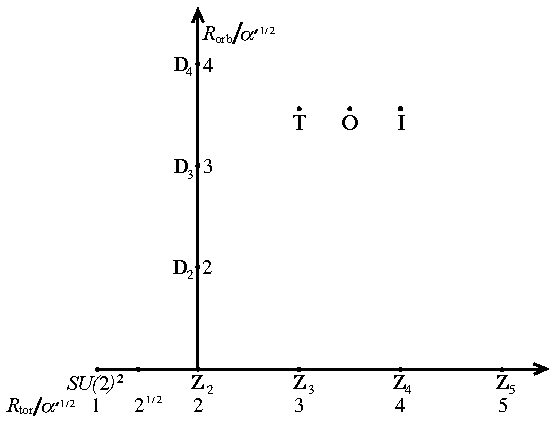
\includegraphics[width=0.78\linewidth]{figures/fig_8_2.pdf}
\caption{$c=1$ の CFT のモジュライ空間。トーラスの枝は水平方向、オービフォールドの枝は垂直方向に伸びる。$SU(2)$ の離散部分群によるツイストから得られる特別な点を示した。これには、正四面体群、正八面体群、正二十面体群から得られる三つの孤立点も含まれる。$R=(2\alpha')^{1/2}$ のトーラスなど、他の特別な半径は後に現れる。}
\label{fig:8.2}
\end{figure}

トーラスの枝とオービフォールドの枝が交わる点の近くの低エネルギー物理を解析すると理解が深まる。この点を、式 (8.5.20) の $r'$ によって $SU(2)$ 理論をツイストしたものとして記述しよう。ツイスト後に残る質量のないスカラーは、$j^3\widetilde j^3$ と、$i,j\in\{1,2\}$ に対する $j^i\widetilde j^j$ である。これらはすべて非ツイストなので、ポテンシャルはツイスト前と同じ $\det M$ である。スカラー場 $M_{ij}$ は再び $U(1)\times U(1)$ 回転によって対角化でき、ちょうど一つの対角成分だけがゼロでない場合にポテンシャルは平坦になる。しかし今度は、モジュラス $M_{33}$ を $M_{11}$ や $M_{22}$ へ回転できないので、これらの方向は物理的に異なる。モジュラス $M_{33}$ は $U(1)\times U(1)$ を破らず、トーラスの枝に沿う移動に対応する。モジュラス $M_{11}$ または $M_{22}$ はゲージ対称性を破り、オービフォールドの枝に沿う移動に対応する。このモジュラスは荷電しているため、その符号反転はゲージ変換である。したがって、物理的に異なるオービフォールドの線は、二つの枝が交わる点で終わる。二つのモジュラスを同時に変化させることはできない。その線形結合はポテンシャルの平坦方向ではないからである。オービフォールド上の弦理論が円上の弦理論と等価になりうるのは非常に驚くべきことであり、弦が時空幾何をわれわれと同じようには見ていないことを、さらに示している。

トーラスの枝に沿って進むと、$SU(2)$ 半径のすべての整数倍 $R=k\alpha'^{1/2}$ に、余分な質量のない状態がある。これらは $(n,w)=(\pm2k,0)$ の状態である。T 双対な記述 $R=\alpha'^{1/2}/k$ において、これらの点は $SU(2)\times SU(2)$ 理論を $\mathbb Z_k$ 対称性
\begin{equation}
X^{25}\longrightarrow X^{25}+\frac{2\pi\alpha'^{1/2}}{k}
\tag{8.5.22}\label{eq:8.5.22}
\end{equation}
でツイストして得られると考えられる。これは $j^1+ij^2$ と $\widetilde j^1+i\widetilde j^2$ に $\exp(2\pi i/k)$ を掛けるので、残る質量のないスカラーは
\begin{equation}
j^3\widetilde j^3,\qquad
j^1\widetilde j^1+j^2\widetilde j^2,\qquad
j^1\widetilde j^2-j^2\widetilde j^1
\tag{8.5.23}\label{eq:8.5.23}
\end{equation}
である。第一のものはトーラスの半径を変えるので、いつものように平坦方向である。しかし、これらの点から別の枝が伸びることはない。$M_{11}=M_{22}$ または $M_{12}=-M_{21}$ の方向では、ポテンシャルが平坦方向をもつための条件 (8.3.23) が満たされないからである。

シフト (8.5.22) は $SU(2)\times SU(2)$ の部分群 $\mathbb Z_k$ を生成する。他の部分群によるツイストを考えよう。シフト (8.5.22) と反射 $X^{25}\to-X^{25}$ が生成する二面体群 $\mathbb D_k$ は、半径 $k\alpha'^{1/2}$ のオービフォールドを与える。他の三つの離散部分群は、正四面体群、正八面体群、正二十面体群である。これらは CFT のモジュライを\textbf{すべて}取り除くので、ツイスト後の CFT は連続な族の一員ではなく、孤立点になる。すべての半径で定義できる $\mathbb Z_k$ および $\mathbb D_k$ ツイストと異なり、これらの離散群は臨界半径にしか存在しない $SU(2)$ の元を含むので、ツイスト後に半径を変えられない。このようなコンパクト空間をもつ弦理論には、スカラーはディラトン一つしかない。以上が知られている $c=1$ の CFT のすべてであり、したがって、知られている25次元のボソン弦背景のすべてを与える。

\subsectionlink{開弦}\label{sec:8.6}

開弦のトーラスコンパクト化に新たに現れるのは、ゲージ場の平坦な背景である、非自明な \textbf{Wilson 線}が可能になることである。まず、いくつかの荷電場を含む $U(1)$ ゲージ理論を調べ、定数背景
\begin{equation}
A_{25}(x^M)=-\frac{\theta}{2\pi R}
=-i\Lambda^{-1}\frac{\partial\Lambda}{\partial x^{25}},
\qquad
\Lambda(x^{25})=\exp\left(-\frac{i\theta x^{25}}{2\pi R}\right)
\tag{8.6.1}\label{eq:8.6.1}
\end{equation}
を考えよう。ここで $\theta$ は定数である。局所的には、これは純粋ゲージである。場の強さはゼロで、場の方程式は自明に満たされる。しかしゲージパラメーター $\Lambda$ は時空の周期性を満たさず、この背景は物理的効果をもつ。それを測るゲージ不変量が Wilson 線
\begin{equation}
W_q=\exp\left(iq\oint dx^{25}\,A_{25}\right)
=\exp(-iq\theta)
\tag{8.6.2}\label{eq:8.6.2}
\end{equation}
である。

まず電荷 $q$ の点粒子を考える。そのゲージ固定した世界線作用は
\begin{equation}
S=\int d\tau\left(\frac12\dot X^M\dot X_M
+\frac{m^2}{2}-iqA_M\dot X^M\right)
\tag{8.6.3}\label{eq:8.6.3}
\end{equation}
である。ゲージ場との作用は単に $-iq\int dx^M A_M$ なので、コンパクト方向を一周する経路は、Wilson 線 $W_q$ に等しい位相を得る。正準運動量は
\begin{equation}
p_{25}=-\frac{\partial L}{\partial v^{25}}
=v^{25}-\frac{q\theta}{2\pi R}
\tag{8.6.4}\label{eq:8.6.4}
\end{equation}
であり、式 (8.4.6) と同様に $v^{25}=i\dot X^{25}$ である。波動関数はコンパクト空間で周期的でなければならないので、整数 $l$ に対して $p_{25}=l/R$ となり、
\begin{equation}
v_{25}=\frac{2\pi l+q\theta}{2\pi R}
\tag{8.6.5}\label{eq:8.6.5}
\end{equation}
を得る。物理的状態を消す Hamiltonian は
\begin{equation}
H=\frac12\left(p_\mu p^\mu+v_{25}^2+m^2\right)
\tag{8.6.6}\label{eq:8.6.6}
\end{equation}
なので、$v_{25}$ が $\theta$ に依存することにより、質量 $-p_\mu p^\mu$ はずれる。同じスペクトルは、粒子ではなく場による記述でも容易に得られる。$v_{25}$ はまさにゲージ不変な運動量 $-i\partial_{25}-qA_{25}$ であることに注意しよう。

ゲージ変換 $\Lambda^{-1}$ によって $A_{25}$ をゼロにしてもよい。このゲージでは、荷電場はもはや周期的でなく、$x^{25}\to x^{25}+2\pi R$ のもとで位相 $\exp(iq\theta)$ を得る。物理的な、すなわちゲージ不変な量は依然として周期的である。今度は正準運動量がずれて、
\begin{equation}
v_{25}=p_{25}=\frac{2\pi l+q\theta}{2\pi R}
\tag{8.6.7}\label{eq:8.6.7}
\end{equation}
となり、ゲージ不変な運動量 $v_{25}$ については先ほどと同じ結果になる。

次に弦に移り、$U(n)$ の Chan--Paton 因子を含めよう。一般の定数 $A_{25}$ はゲージ変換で対角化でき、
\begin{equation}
A_{25}=-\frac1{2\pi R}\operatorname{diag}(\theta_1,\theta_2,\ldots,\theta_n)
\tag{8.6.8}\label{eq:8.6.8}
\end{equation}
となる。ゲージ場は $U(n)$ の対角部分群、すなわち $U(1)^n$ に属する。ゲージ場は一般の状態の Chan--Paton 因子に $[A_M,\lambda]$ として結合するので、Chan--Paton 状態 $|ij\rangle$ にある弦は、$U(1)_i$ のもとで電荷 $+1$、$U(1)_j$ のもとで電荷 $-1$ をもち、他の因子に対しては中性である。したがって、
\begin{equation}
v_{25}=\frac{2\pi l-\theta_j+\theta_i}{2\pi R}
\tag{8.6.9}\label{eq:8.6.9}
\end{equation}
となる。開弦のスペクトルは
\begin{equation}
m^2=\frac{(2\pi l-\theta_j+\theta_i)^2}{4\pi^2R^2}
+\frac1{\alpha'}(N-1)
\tag{8.6.10}\label{eq:8.6.10}
\end{equation}
である。

特にゲージボソンを考えると、$l=0$、$N=1$ なので、
\begin{equation}
m^2=\frac{(\theta_j-\theta_i)^2}{4\pi^2R^2}
\tag{8.6.11}\label{eq:8.6.11}
\end{equation}
となる。一般の背景では、すべての $\theta$ が異なり、質量のないベクトルは $i=j$ の対角成分だけである。この場合、破れていないゲージ群は $U(1)^n$ である。$r$ 個の $\theta$ が等しければ、対応する $r\times r$ 行列のベクトルが質量を失い、$U(r)$ ゲージ対称性を担う。$n$ 個の $\theta$ が、それぞれ $r_i$ 個ずつ等しい組に分かれるとき、ゲージ対称性は
\begin{equation}
U(r_1)\times\cdots\times U(r_s),\qquad
\sum_{i=1}^{s}r_i=n
\tag{8.6.12}\label{eq:8.6.12}
\end{equation}
となる。

いつものように、低エネルギーでの解釈がある。ゲージ場 $A_{25}$ は $U(n)$ の随伴表現に属する25次元スカラーであり、その真空期待値が対称性を自発的に $U(r_1)\times\cdots\times U(r_s)$ へ破る。低エネルギー有効作用の詳細は読者に委ねる。重要なのは、コンパクト方向が $k$ 個あるとき、ポテンシャルに、26次元 Yang--Mills 作用の場の強さから来る項
\begin{equation}
\operatorname{Tr}\left([A_m,A_n]^2\right)
\tag{8.6.13}\label{eq:8.6.13}
\end{equation}
が含まれることである。このため、静的解では異なる方向のゲージ場は可換でなければならず、同時に対角化できる。したがって、ゲージ場から $kn$ 個、計量と反対称テンソルから $k^2$ 個のモジュライが得られる。

\subsubsectionlink*{T 双対性}

開弦スペクトルの $R\to0$ 極限を考えよう。Neumann 境界条件をもつ開弦には、$w$ に相当する量子数がない。周期方向の巻き付きを常にほどけるからである。したがって $R\to0$ では、運動量がゼロでない状態の質量は無限大になるが、新たな連続状態は現れない。振る舞いは場の理論と同じで、残る状態は25次元時空を運動する。

開弦を含む理論には必ず閉弦もあることを思い出すと、一見したところ逆説が生じる。$R\to0$ 極限で閉弦は26次元時空を運動するのに、開弦は25次元しか運動しないからである。何が起きているかは、次のように考えられる。開弦の内部は閉弦と同じ「物質」からできているので、依然として26次元で振動しているはずである。開弦を特徴付けるものは端点なので、25次元の超平面に制限されなければならないのは、この端点である。

\begin{figure}[tbp]
\centering
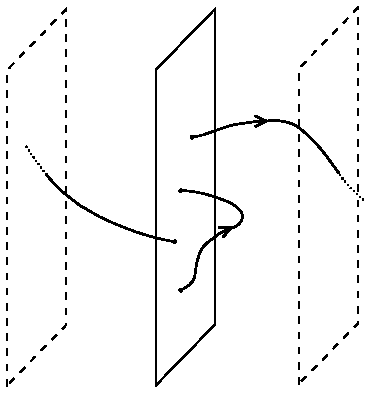
\includegraphics[width=0.62\linewidth]{figures/fig_8_3.pdf}
\caption{端点が超平面に付いた開弦。破線の平面は周期的に同一視されている。巻き付き数が0と1の二本の弦を示す。}
\label{fig:8.3}
\end{figure}

実際、T 双対理論を、新しい埋め込み座標
\begin{equation}
X'^{25}(z,\bar z)=X_L^{25}(z)-X_R^{25}(\bar z)
\tag{8.6.14}\label{eq:8.6.14}
\end{equation}
を使って記述することを思い出そう。このとき
\begin{equation}
\partial_nX^{25}=-i\partial_tX'^{25}
\tag{8.6.15}\label{eq:8.6.15}
\end{equation}
であり、$n$ は境界に垂直、$t$ は境界に接する方向を表す。元の座標に対する Neumann 条件は、双対座標に対する Dirichlet 条件である。すなわち、弦の各端点の $X'^{25}$ 座標が固定される。

まず Wilson 線のないコンパクト化を考えよう。この場合、実はすべての端点が\textbf{同じ}超平面上に拘束される。これを見るために、次を積分する。
\begin{equation}
\begin{split}
X'^{25}(\pi)-X'^{25}(0)
&=\int_0^\pi d\sigma^1\,\partial_1X'^{25}
=-i\int_0^\pi d\sigma^1\,\partial_2X^{25}\\
&=-2\pi\alpha'v^{25}
=-\frac{2\pi\alpha'l}{R}=-2\pi lR'.
\end{split}
\tag{8.6.16}\label{eq:8.6.16}
\end{equation}
両端の間での $X'^{25}$ の変化は、双対方向の周期 $2\pi R'$ の整数倍なので、周期的な T 双対空間では両端は同じ超平面にある。二本の\textbf{異なる}開弦については、それらの間の重力子交換によって得られる連結な世界面を考えよう。任意の二つの端点を結ぶ経路に沿って、同じ議論 (8.6.16) を適用できる。したがって図8.3のように、すべての弦のすべての端点は同じ超平面上にある。他の24個の空間方向では、端点は依然として自由に動ける。

\begin{figure}[tbp]
\centering
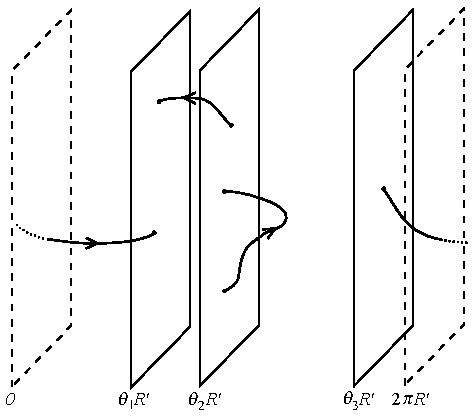
\includegraphics[width=0.72\linewidth]{figures/fig_8_4.pdf}
\caption{異なる位置にある $n=3$ 枚の超平面と、それらに付いたさまざまな弦。タキオンを無視すると、両端が同じ超平面上にある最も軽い弦は質量がない。一方、一致しない超平面間に張られた弦は、その張力のために質量をもつ。二つの超平面が一致すると、それらの間に張られた最も軽い弦は質量を失う。}
\label{fig:8.4}
\end{figure}

次に Wilson 線の効果を考える。$v_{25}$ のシフト (8.6.9) によって、差 (8.6.16) は
\begin{equation}
\Delta X'^{25}=X'^{25}(\pi)-X'^{25}(0)
=-(2\pi l-\theta_j+\theta_i)R'
\tag{8.6.17}\label{eq:8.6.17}
\end{equation}
に置き換わる。言い換えると、任意の加法定数を除いて、状態 $i$ の端点の位置は
\begin{equation}
X'^{25}=\theta_iR'=-2\pi\alpha'A_{25,ii}
\tag{8.6.18}\label{eq:8.6.18}
\end{equation}
である。したがって一般に、図8.4に示すように、異なる位置に $n$ 枚の超平面がある。

Chan--Paton 状態 $|ij\rangle$ をもち、コンパクト方向に $l$ 回巻き付く開弦のセクターでのモード展開は、
\begin{equation}
\begin{split}
X'^{25}(z,\bar z)
={}&\theta_iR'-\frac{iR'}{2\pi}(2\pi l-\theta_j+\theta_i)\ln(z/\bar z)\\
&+i\left(\frac{\alpha'}2\right)^{1/2}
\sum_{\substack{m=-\infty\\m\ne0}}^\infty
\frac{\alpha_m^{25}}{m}(z^{-m}-\bar z^{-m})\\
={}&\theta_iR'+\frac{\sigma^1}{\pi}\Delta X'^{25}
-(2\alpha')^{1/2}
\sum_{\substack{m=-\infty\\m\ne0}}^\infty
\frac{\alpha_m^{25}}{m}\exp(-m\sigma^2)\sin m\sigma^1.
\end{split}
\tag{8.6.19}\label{eq:8.6.19}
\end{equation}
スペクトル (8.6.10) は
\begin{equation}
m^2=\left(\frac{\Delta X'^{25}}{2\pi\alpha'}\right)^2
+\frac1{\alpha'}(N-1)
\tag{8.6.20}\label{eq:8.6.20}
\end{equation}
となる。ここで式 (8.6.17) で与えられる $\Delta X'^{25}$ は、与えられたセクターの弦の最小長さである。

例えば $p+1\leq m\leq25$ に対する $X^m$ のように、複数の座標が周期的であり、それらの方向を双対座標で書き直す場合に、この描像がどのように一般化されるかを考えよう。$X^m$ の Neumann 条件は再び双対座標 $X'^m$ の Dirichlet 条件になるので、開弦の端点は、平行な $n$ 個の $(p+1)$ 次元部分空間に閉じ込められる。各方向の Wilson 線は、各部分空間の独立な座標となる。

双対な描像は、開弦の境界条件によって並進不変性が破れているという点で、いささか奇妙である。これは単に、元の開弦理論では巻き付き数が保存されないことを反映している。巻き付いた閉弦は切れて開き、巻き付きをほどける。そして巻き付き数は、T 双対性によって運動量に対応する。T 双対性は同じ理論の異なる記述にすぎず、さらに、元の理論のコンパクト化半径が小さいときには、T 双対な描像を使うのが自然であることを覚えておく必要がある。この場合、図8.4が、得られる物理をどのように解釈すればよいかを示している。

\subsectionlink{D ブレーン}\label{sec:8.7}

開弦理論を小さなトーラス上にコンパクト化すると、その物理は、大きなトーラスへのコンパクト化において、開弦の端点を部分空間上に制限したものとして記述されることがわかった。実は、これらの部分空間は、それ自体が新しい力学的な対象である。簡単のため、双対化する座標が一つだけの場合を取り、すべての $\theta_i$ が異なる一般の配置における、質量のない開弦のスペクトルを考えよう。タキオンを無視すると、質量 (8.6.20) がゼロになるのは $N=1$、$\Delta X'^{25}=0$ の場合だけである。すなわち、両端は同じ超平面上にあり、巻き付き数はゼロである。したがって、質量のない状態
\begin{align}
&\alpha_{-1}^\mu|k;ii\rangle,\qquad
\mathcal V=i\partial_tX^\mu,
\tag{8.7.1a}\label{eq:8.7.1a}\\
&\alpha_{-1}^{25}|k;ii\rangle,\qquad
\mathcal V=i\partial_tX^{25}=\partial_nX'^{25}
\tag{8.7.1b}\label{eq:8.7.1b}
\end{align}
が得られる。

もちろん、これらは元の理論と同じ質量のない状態であり、T 双対性は同じスペクトルに別の描像を与えるだけである。一般の Wilson 線の場合、元の理論における質量のない開弦状態は、$n$ 個の質量のない $U(1)$ ベクトルだけだった。式 (8.7.1) では、それらを偏極が超平面に接するか、垂直かによって分けた。接する偏極をもつ25個の状態は、超平面上に存在するゲージ場をなす。垂直な偏極をもつ状態は、元の理論ではコンパクト方向のゲージ場であったが、T 双対理論では単純かつ重要な解釈をもつ。それは超平面の形状に対する\textbf{集団座標}である。定数のゲージ背景 (8.6.18) が超平面の一様な並進に対応することから、これはすでに明らかである。同じ理由で、$x^\mu$ に依存する背景は $x^\mu$ に依存する並進、すなわち曲がった超平面へ移り、場 $A_{ii}^{25}$ の量子は、超平面の小さな振動に対応する。

これは時空そのものに起きたのと同じ現象である。平坦な背景における弦から始めて、ある質量のない閉弦状態が幾何の揺らぎに対応すると発見した。ここでは、まず超平面が現れ、次に、ある開弦状態がその形状の揺らぎに対応するとわかった。超平面が力学的になったことは、驚くべきではない。弦理論は重力を含む。超平面を通過する重力波は時空そのものを歪めるので、超平面だけが剛体のままでいるとは考えにくい。

したがって、この超平面は確かに力学的な対象であり、\textbf{Dirichlet 膜}、略して\textbf{D ブレーン}である。$25-p$ 個の方向を双対化して得られる $p$ 次元 D ブレーンを D$p$ ブレーンと呼ぶ。この用語では、元の $U(n)$ 開弦理論には $n$ 枚の D25 ブレーンが含まれる。D25 ブレーンは空間を満たすので、弦の端点はどこにあってもよい。これは通常の Chan--Paton 因子に対応するだけである。

T 双対性は Neumann 境界条件と Dirichlet 境界条件を入れ替えるので、D$p$ ブレーンに接する方向でさらに T 双対変換すると、D$(p-1)$ ブレーンになる。一方、垂直な方向の T 双対変換では D$(p+1)$ ブレーンになる。自明でない角度をなす場合は、まもなく現れる。

Dirichlet 境界条件を、それ自体として調べるところから始めることもできた。ここで採った、T 双対性を通してそれを発見する道筋は、その多くの性質を導くのに適している。またこれは、「通常の」状態から連続的な過程によって、D ブレーンを含む状態に到達できることも示している。すなわち、元の理論の $R\to0$ 極限を取れば、非コンパクト空間に D ブレーンが残る。超弦では、このことを用いて、D ブレーンが理論の非摂動的定義に不可欠な要素であると論じる。ボソン弦については、この議論を試みない。理論が非摂動的な定義をもつという強い根拠がないからである。ボソン弦理論は、超弦理論の一部を切り落としたものとしてしか存在しないのかもしれない。

$U(n)$ の対称性の破れを、T 双対な描像で見るのは興味深い。どの D ブレーンも一致していないとき、各ブレーンには質量のないベクトルが一つだけあり、全体のゲージ群は $U(1)^n$ となる。$r$ 枚の D ブレーンが一致すると、それらの間に張られた弦の長さがゼロになれるため、新たな質量のない状態が現れる。質量公式 (8.6.20) の $\Delta X'^{25}$ は、$i,j$ の両方がこの $r$ 枚の集合に属していれば、$n=0$ でゼロになる。したがって、$U(r)$ ゲージ群の随伴表現をなす $r^2$ 個のベクトルがある。これは双対な Wilson 線の描像で見いだしたものと同じである。しかし注目すべきことに、D ブレーンに垂直な成分から、質量のないスカラーも $r^2$ 個現れる。この意味は以下で論じる。

\subsubsectionlink*{D ブレーン作用}

D$p$ ブレーンの世界体積上の質量のない場は、$U(1)$ ベクトルと、揺らぎを記述する $25-p$ 個の世界ブレーン上のスカラーである。この系の低エネルギー有効作用を考えることは、いつものように非常に有用である。ここで双対半径 $R'$ を無限大にし、得られる26次元時空の中の一枚の D ブレーンに注目する。世界ブレーン上の場は、第3.7節ですでに作用を論じた、質量のない閉弦場と相互作用している。ブレーン上に座標 $\xi^a$、$a=0,\ldots,p$ を導入する。ブレーン上の場は埋め込み $X^\mu(\xi)$ とゲージ場 $A_a(\xi)$ である。作用は
\begin{equation}
\boldsymbol S_p=-T_p\int d^{p+1}\xi\,e^{-\Phi}
\left[-\det(G_{ab}+B_{ab}+2\pi\alpha'F_{ab})\right]^{1/2}
\tag{8.7.2}\label{eq:8.7.2}
\end{equation}
であると主張する。$T_p$ は後で決定する定数である。ここで、
\begin{equation}
\begin{split}
G_{ab}(\xi)&=\frac{\partial X^\mu}{\partial\xi^a}
\frac{\partial X^\nu}{\partial\xi^b}G_{\mu\nu}(X(\xi)),\\
B_{ab}(\xi)&=\frac{\partial X^\mu}{\partial\xi^a}
\frac{\partial X^\nu}{\partial\xi^b}B_{\mu\nu}(X(\xi))
\end{split}
\tag{8.7.3}\label{eq:8.7.3}
\end{equation}
は、ブレーン上の誘導計量と誘導反対称テンソルである。

作用 (8.7.2) の特徴はすべて、一般的な考察から理解できる。まず時空計量と埋め込みだけを考えると、最も単純で微分の次数が最も低い、座標不変な作用は、世界体積 $(-\det G_{ab})^{1/2}$ の積分である。これは誘導場 (8.7.3) を通して $X^\mu(\xi)$ に暗黙に依存することに注意しよう。平坦な D ブレーンのまわりで展開すると、Nambu--Goto 作用が弦の揺らぎを記述するのと同様に、揺らぎの作用を与える。

ディラトン依存性 $e^{-\Phi}\propto g_{\mathrm c}^{-1}$ は、これが開弦の木レベル作用であるために現れる。開弦場の自己相互作用も、閉弦場への結合も、まず円板から生じる。

$F_{ab}$ への依存性は T 双対性を用いて理解できる。$X^1$ 方向と $X^2$ 方向に伸びる D ブレーンを考え、他の方向は指定しないことにし、その上に定数のゲージ場 $F_{12}$ があるとする。$A_2=X^1F_{12}$ のゲージに移ろう。次に2方向で T 双対変換する。この方向の Neumann 条件は Dirichlet 条件に置き換わるので、D ブレーンの次元は一つ減る。しかし、ポテンシャルと座標の間の T 双対関係 (8.6.18) から、D ブレーンは $(1\text{--}2)$ 平面内で傾き、
\begin{equation}
X'^2=-2\pi\alpha'X^1F_{12}
\tag{8.7.4}\label{eq:8.7.4}
\end{equation}
となる。この傾きは、作用に幾何学的因子
\begin{equation}
\int dX^1\left[1+(\partial_1X'^2)^2\right]^{1/2}
=\int dX^1\left[1+(2\pi\alpha'F_{12})^2\right]^{1/2}
\tag{8.7.5}\label{eq:8.7.5}
\end{equation}
を与える。

任意の D ブレーンに対して、ブーストで座標軸にそろえ、次に回転で $F_{ab}$ をブロック対角形にすれば、作用を各平面の因子 (8.7.5) の積へ帰着できる。これは行列式 (8.7.2) 中の $F_{ab}$ 項と等価である。この行列式の形をしたゲージ場の作用は Born--Infeld 作用として知られる。当初は、量子電磁力学の短距離発散の解決として提案されたが、その目的では成功しなかった。

最後に、$B_{ab}$ への依存性は次の議論で与えられる。閉弦場 $B_{\mu\nu}$ と開弦場 $A^\mu$ は、弦の世界面作用に次の形で現れる。\footnote[3]{微分形式に詳しい読者のために書くと、これは
\[
\frac{i}{2\pi\alpha'}\int_M B+i\int_{\partial M}A
\]
である。以下の式も同様に書き直せる。}
\begin{equation}
\frac{i}{4\pi\alpha'}\int_M d^2\sigma\,g^{1/2}
\epsilon^{ab}\partial_aX^\mu\partial_bX^\nu B_{\mu\nu}
+i\int_{\partial M}dX^\mu A_\mu.
\tag{8.7.6}\label{eq:8.7.6}
\end{equation}
これらの場にはそれぞれ時空のゲージ不変性があり、時空理論の整合性のために、それらを保たなければならない。通常のゲージ変換
\begin{equation}
\delta A_\mu=\partial_\mu\lambda
\tag{8.7.7}\label{eq:8.7.7}
\end{equation}
は作用 (8.7.6) の対称性である。境界項の変化が全微分の積分だからである。反対称テンソルの変換
\begin{equation}
\delta B_{\mu\nu}=\partial_\mu\zeta_\nu-\partial_\nu\zeta_\mu
\tag{8.7.8}\label{eq:8.7.8}
\end{equation}
も同様に、バルク作用を全微分だけ変えるが、境界をもつ世界面では、これは表面項を生む。これを打ち消すには、開弦場 $A_\mu$ もテンソルのゲージ対称性のもとで
\begin{equation}
\delta A_\mu=-\frac{\zeta_\mu}{2\pi\alpha'}
\tag{8.7.9}\label{eq:8.7.9}
\end{equation}
と変換しなければならない。しかしこのとき、両方の対称性のもとで不変なのは組合せ
\begin{equation}
B_{\mu\nu}+2\pi\alpha'F_{\mu\nu}
\equiv2\pi\alpha'\mathcal F_{\mu\nu}
\tag{8.7.10}\label{eq:8.7.10}
\end{equation}
だけであり、作用にはこの組合せが現れなければならない。こうして作用の形 (8.7.2) が完全に決まる。

確認として、$G_{\mu\nu}+B_{\mu\nu}$ という組合せが現れるのは自然である。同じ組合せが共形ゲージの世界面作用に現れるからである。なお、作用 (8.7.2) は、さまざまな開弦振幅および開弦と閉弦を含む振幅の低エネルギー極限を取ることによっても求められるが、その方が手間はかかる。

互いに離れた $n$ 枚の D ブレーンについては、作用は単一の D ブレーンの作用を $n$ 個足したものである。しかし、D ブレーンが一致すると、ブレーン上の質量のないベクトルとスカラーは $n$ 個でなく $n^2$ 個になることを見た。これらを支配する有効作用を書きたい。今や場 $X^\mu(\xi)$ と $A_a(\xi)$ は $n\times n$ 行列である。ゲージ場についての意味は明らかで、非 Abel な $U(n)$ ゲージ場になる。しかし集団座標 $X^\mu$ についての意味は謎めいている。時空への $n$ 枚の D ブレーンの埋め込みを表す集団座標が、$n\times n$ 行列へ拡大されているのである。この「非可換幾何」が D ブレーンの力学に重要な役割を果たすことは明らかになっており、時空の本性に関する重要な手がかりであるとの推測もある。

有効作用を考えると、さらに理解が進む。今度は作用に微分を含まない項、すなわち集団座標のポテンシャルがあり、これは定数の $A_m$ 場から T 双対性によって導ける。このようなベクトルポテンシャルでは、場の強さは単に $[A_m,A_n]$ であり、T 双対な描像では $(2\pi\alpha')^{-2}[X_m,X_n]$ になる。場の強さで展開すると、作用の先頭項は概略
\begin{equation}
V\propto\operatorname{Tr}\left([X_m,X_n][X^m,X^n]\right)
\tag{8.7.11}\label{eq:8.7.11}
\end{equation}
となる。このポテンシャルは、点 $X^m=0$ において二階微分がゼロになるので、$kn^2$ 個のスカラーはすべて質量がない。ここでも $k=25-p$ は双対化した方向の数である。しかし平坦方向の空間は、それより小さい。ポテンシャルは二乗の和なので、すべての $[X^m,X^n]$ がゼロである場合に限ってゼロになる。その場合には、$U(n)$ ゲージ対称性を使って、すべての $X^m$ が対角となるゲージへ移れる。したがって平坦方向は、対角成分の個数に等しい $kn$ 個である。これら $kn$ 個の対角成分は、$n$ 枚の D$p$ ブレーンの集団座標と解釈できる。ゆえにポテンシャル (8.7.11) は、離れた D ブレーンと一致した D ブレーンの物理を正しくつなぐ。

$X^m$ が可換な場合、作用は互いに離れた $n$ 枚の D ブレーンの作用に帰着しなければならないので、
\begin{equation}
\begin{split}
\boldsymbol S_p=-T_p\int d^{p+1}\xi\,
\operatorname{Tr}\bigl\{&
e^{-\Phi}[-\det(G_{ab}+B_{ab}+2\pi\alpha'F_{ab})]^{1/2}\\
&+O([X^m,X^n]^2)\bigr\}
\end{split}
\tag{8.7.12}\label{eq:8.7.12}
\end{equation}
でなければならない。行列式は世界体積の添字 $ab$ に関して取り、トレースは $n$ 個の Chan--Paton 添字に関して取る。このトレースは適切な $U(n)$ 不変量であり、対角行列の場合には個々の D ブレーンについての和に帰着する。交換子への完全な依存性は、単純なポテンシャル (8.7.11) より複雑で、他の場への追加の結合や、交換子の高次の補正がある。しかし重要な性質、すなわち平坦方向の形は変わらない。完全な依存性は、すべての方向が Neumann 条件を満たす場合の Born--Infeld 作用から出発して、T 双対変換を行うことで求められる。なお、場の強さの交換子を含む高階微分項は、T 双対性だけでは決定できない。

\subsubsectionlink*{D ブレーンの張力}

定数 $T_p$ を計算することは理解を深めるうえで有用であり、超弦ではその正確な値が重要になる。具体的な計算を行う前に、T 双対性から $T_p$ の漸化式が得られることに注目しよう。ディラトンが定数の背景では、D$p$ ブレーンの張力は $T_pe^{-\Phi}$ である。これは静的な D ブレーンの単位体積あたりの作用に負号を付けたものだからである。ここで D$p$ ブレーンに接する $p$ 個の方向が周期的に同一視されている場合を考えよう。すなわち、D$p$ ブレーンは時空内の $p$ 次元トーラスに\textbf{巻き付いている}。その質量は張力とトーラスの体積の積
\begin{equation}
T_pe^{-\Phi}\prod_{i=1}^{p}(2\pi R_i)
\tag{8.7.13}\label{eq:8.7.13}
\end{equation}
である。周期方向の一つ $X^p$ で T 双対変換しよう。これは同じ状態の新しい記述にすぎないので、質量を変えない。T 双対理論のディラトン (8.3.31) を用いると、質量 (8.7.13) は
\begin{equation}
2\pi\alpha'^{1/2}T_pe^{-\Phi'}
\prod_{i=1}^{p-1}(2\pi R_i)
\tag{8.7.14}\label{eq:8.7.14}
\end{equation}
となる。しかし双対理論では、これは $(p-1)$ 次元トーラスに巻き付いた D$(p-1)$ ブレーンなので、その質量は
\begin{equation}
T_{p-1}e^{-\Phi'}\prod_{i=1}^{p-1}(2\pi R_i)
\tag{8.7.15}\label{eq:8.7.15}
\end{equation}
である。質量 (8.7.14) と (8.7.15) を等置すると、
\begin{equation}
T_p=\frac{T_{p-1}}{2\pi\alpha'^{1/2}}
\tag{8.7.16}\label{eq:8.7.16}
\end{equation}
を得る。これによって、全体の規格化定数一つを除いて $T_p$ が決まる。

\begin{figure}[tbp]
\centering
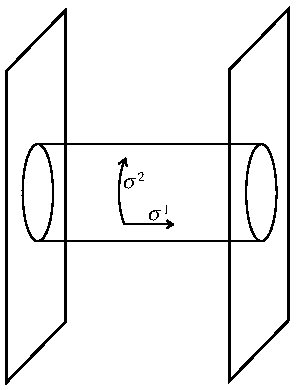
\includegraphics[width=0.64\linewidth]{figures/fig_8_5.pdf}
\caption{二枚の D ブレーン間の閉弦交換。等価に、各 D ブレーンに片端ずつ付いた開弦の真空ループである。}
\label{fig:8.5}
\end{figure}

D ブレーンの張力の実際の値を決めるには、弦振幅を計算する必要がある。例えば、重力子の頂点演算子をもつ円板で与えられる、D ブレーンへの重力結合から求めてもよい。しかし、そこにはまだわかっていない比 $g_{\mathrm c}/g_{\mathrm o}^2$ が含まれる。閉弦結合は頂点演算子から、開弦結合は円板から現れる。代わりに、次のように絶対的な規格化を求められる。位置 $X_1^m=0$ と $X_2^m=y^m$ にある、平行な二枚の D$p$ ブレーンを考えよう。この二つの対象は、図8.5のように閉弦を交換することで互いの存在を感じる。この弦振幅は頂点演算子をもたないアニュラスなので、前章と同じ方法で計算できる。重力子とディラトンの交換による極から、閉弦状態の D ブレーンへの結合 $T_p$ が得られる。

第7.4節では、アニュラスの真空振幅を開弦のループとして計算したが、モジュライ積分の $t\to0$ 極限から閉弦の極が見つかったことを思い出そう。ここで関心があるのはまさにそれらの極だが、振幅を計算する最も簡単な方法は、やはり開弦のループとみなすことである。実際、先の結果 (7.4.1) は、わずかな変更だけで適用できる。運動量積分の数は26から $p+1$ へ減り、それに応じて $V_{26}$ は $V_{p+1}$ になる。ウェイト $h_i$ には、伸びた弦の張力から $y^2/(4\pi^2\alpha')$ が加わる。Chan--Paton のウェイト $n^2$ は2になる。弦はどちらの向きにも付けられるからである。したがって、
\begin{equation}
\begin{split}
\mathcal A
&=iV_{p+1}\int_0^\infty\frac{dt}{t}
(8\pi^2\alpha't)^{-(p+1)/2}
\exp(-ty^2/2\pi\alpha')\eta(it)^{-24}\\
&=\frac{iV_{p+1}}{(8\pi^2\alpha')^{(p+1)/2}}
\int_0^\infty dt\,t^{(21-p)/2}\exp(-ty^2/2\pi\alpha')\\
&\qquad\times\left[\exp(2\pi/t)+24+\cdots\right]
\end{split}
\tag{8.7.17}\label{eq:8.7.17}
\end{equation}
を得る。漸近形は、第7.4節とまったく同様にして求めた。第一項はタキオン交換から来るので、やはりボソン弦特有の、ここでは関心のない効果である。第二項を積分すると、
\begin{equation}
\begin{split}
\mathcal A
&=iV_{p+1}\frac{24}{2^{12}}(4\pi^2\alpha')^{11-p}
\pi^{(p-23)/2}\Gamma\left(\frac{23-p}{2}\right)|y|^{p-23}\\
&=iV_{p+1}\frac{24\pi}{2^{10}}(4\pi^2\alpha')^{11-p}G_{25-p}(y)
\end{split}
\tag{8.7.18}\label{eq:8.7.18}
\end{equation}
を得る。$G_d(y)$ は $d$ 次元の質量のないスカラーの Green 関数、すなわち $-\nabla^2$ の逆である。

次に、これを同じ振幅の場の理論による計算と比較する必要がある。反対称テンソルは D ブレーンに結合しないので、時空作用 (3.7.25) の関係する項は
\begin{equation}
\boldsymbol S=\frac1{2\kappa^2}\int d^{26}X\,(-\widetilde G)^{1/2}
\left(\widetilde{\boldsymbol R}
-\frac16\widetilde\nabla_\mu\widetilde\Phi\,
\widetilde\nabla^\mu\widetilde\Phi\right)
\tag{8.7.19}\label{eq:8.7.19}
\end{equation}
である。チルダは Einstein 計量を表すことを思い出そう。この形は、その作用がディラトンの作用から分離するため便利である。チルダの付いたディラトンは、期待値がゼロになるようシフトしてある。同じ変数を使うと、D ブレーン作用 (8.7.2) の関係する項は
\begin{equation}
\boldsymbol S_p=-\tau_p\int d^{p+1}\xi\,
\exp\left(\frac{p-11}{12}\widetilde\Phi\right)
(-\det\widetilde G_{ab})^{1/2}
\tag{8.7.20}\label{eq:8.7.20}
\end{equation}
となる。$\tau_p=T_pe^{-\Phi_0}$ と定義した。これは、ディラトンの背景値が $\Phi_0$ のときの D$p$ ブレーンの実際の物理的張力である。

図8.5に対応する場の理論のグラフは、D ブレーン間の一個の重力子またはディラトンの交換である。伝播関数を求めるために、時空作用を $h_{\mu\nu}=\widetilde G_{\mu\nu}-\eta_{\mu\nu}$ の二次まで、また $\widetilde\Phi$ の二次まで展開する。重力の計算では、ゲージも選ばなければならない。摂動計算に最も簡単なゲージは
\begin{equation}
F_\nu\equiv\partial^{\widehat\mu}h_{\mu\nu}
-\frac12\partial_\nu h^{\widehat\mu}{}_\mu=0
\tag{8.7.21}\label{eq:8.7.21}
\end{equation}
である。ハットは、平坦時空の計量 $\eta^{\mu\nu}$ によって添字を上げたことを表す。作用を二次まで展開し、ゲージ固定項 $-F_\nu F^{\widehat\nu}/(4\kappa^2)$ を加えると、時空作用は
\begin{equation}
\boldsymbol S=-\frac1{8\kappa^2}\int d^{26}X
\left(
\partial_\mu h_{\nu\lambda}\partial^{\widehat\mu}h^{\widehat\nu\widehat\lambda}
-\frac12\partial_\mu h^{\widehat\nu}{}_\nu
\partial^{\widehat\mu}h^{\widehat\lambda}{}_\lambda
+\frac23\partial_\mu\widetilde\Phi\,
\partial^{\widehat\mu}\widetilde\Phi
\right)
\tag{8.7.22}\label{eq:8.7.22}
\end{equation}
となる。運動項を反転すると、運動量空間の伝播関数
\begin{align}
\langle\widetilde\Phi\widetilde\Phi\rangle
&=-\frac{(D-2)i\kappa^2}{4k^2},
\tag{8.7.23a}\label{eq:8.7.23a}\\
\langle h_{\mu\nu}h_{\sigma\rho}\rangle
&=-\frac{2i\kappa^2}{k^2}
\left(\eta_{\mu\sigma}\eta_{\nu\rho}
+\eta_{\mu\rho}\eta_{\nu\sigma}
-\frac2{D-2}\eta_{\mu\nu}\eta_{\sigma\rho}\right)
\tag{8.7.23b}\label{eq:8.7.23b}
\end{align}
を得る。後で参照するため、一般の $D$ に対する形を示した。平坦な配置のまわりで展開した D ブレーン作用は
\begin{equation}
\boldsymbol S_p=-\tau_p\int d^{p+1}\xi
\left(\frac{p-11}{12}\widetilde\Phi-\frac12h_{aa}\right)
\tag{8.7.24}\label{eq:8.7.24}
\end{equation}
である。ここで $h_{\mu\nu}$ のトレースは、D ブレーンに接する方向だけについて取っていることに注意しよう。$\xi$ は、計量 $\delta_{ab}$ をもつ直交直線座標に取った。

これで Feynman グラフを読み取れる。
\begin{equation}
\begin{split}
\mathcal A
&=\frac{i\kappa^2\tau_p^2}{k_\perp^2}V_{p+1}
\left\{6\left[\frac{p-11}{12}\right]^2
+\frac12\left[2(p+1)-\frac1{12}(p+1)^2\right]\right\}\\
&=\frac{6i\kappa^2\tau_p^2}{k_\perp^2}V_{p+1}.
\end{split}
\tag{8.7.25}\label{eq:8.7.25}
\end{equation}
弦の結果 (8.7.18) と比較すると、
\begin{equation}
\tau_p^2=\frac{\pi}{256\kappa^2}(4\pi^2\alpha')^{11-p}
\tag{8.7.26}\label{eq:8.7.26}
\end{equation}
が得られる。計算を整理した結果が T 双対性からの漸化式を満たすことは、有用な確認となる。

一つの応用として、$n$ 枚の25ブレーンをもつ状態を考えよう。これは、通常の、すべての方向が Neumann 条件を満たす $n$ 値の Chan--Paton 因子と同じである。25ブレーン作用 (8.7.12) をゲージ場の二次まで展開すると、
\begin{equation}
\frac{\tau_{25}}4(2\pi\alpha')^2
\operatorname{Tr}(F_{\mu\nu}F^{\mu\nu})
\tag{8.7.27}\label{eq:8.7.27}
\end{equation}
を得る。これは開弦のゲージ結合と重力結合を関係付ける。式 (6.5.14)、(6.5.16)、(6.6.15)、(6.6.18) を用いれば、頂点演算子の規格化 $g_{\mathrm c}$ と $g_{\mathrm o}$ の関係として、
\begin{equation}
\frac{g_{\mathrm o}^2}{g_{\mathrm c}}
=\frac{4\pi\alpha'g_{\mathrm o}'{}^2}{\kappa}
=2^{18}\pi^{25/2}\alpha'^6
\tag{8.7.28}\label{eq:8.7.28}
\end{equation}
と書ける。これは、開弦結合の二乗が閉弦結合に比例するという正しい形をもち、今度は数値係数も含まれている。本質的には、アニュラス図の閉弦の極で因数分解することによって、ユニタリティからこの結果を得た。演習7.9のように、D ブレーンを経由せず、より直接に求めることもできた。

\subsectionlink{向きのない理論の T 双対性}\label{sec:8.8}

向きのない弦理論の $R\to0$ 極限も、興味深い新しい物理をもたらす。まず閉弦を考えよう。向きのない理論を作るには、状態に $\Omega=+1$ を課す。第8.5節の議論に従えば、これは $\Omega$ のゲージ化と考えられる。特に、世界面を組み立てる際の遷移関数には、今や向きの反転を含めてよい。これはゲージ対称性だからであり、こうして向きのない世界面が生まれる。

T 双対理論は、$X^m(z,\bar z)=X_L^m(z)+X_R^m(\bar z)$ の代わりに、座標 $X'^m(z,\bar z)=X_L^m(z)-X_R^m(\bar z)$ を用いることで得られる。元の記述では、世界面パリティ $\Omega$ をゲージ化しており、その作用は
\begin{equation}
\Omega:\quad X_L^M(z)\longleftrightarrow X_R^M(z)
\tag{8.8.1}\label{eq:8.8.1}
\end{equation}
である。T 双対座標で表すと、これは
\begin{align}
\Omega:\quad X'^m(z,\bar z)&\longleftrightarrow-X'^m(\bar z,z),
\tag{8.8.2a}\label{eq:8.8.2a}\\
X^\mu(z,\bar z)&\longleftrightarrow X^\mu(\bar z,z)
\tag{8.8.2b}\label{eq:8.8.2b}
\end{align}
となる。ここでも $m$ は T 双対化した座標、$\mu$ は双対化していない座標を表す。したがって双対な描像では、対称性 (8.8.2) は世界面パリティ変換と時空反射の積である。世界面パリティだけをゲージ化すると向きのない理論が得られ、反射だけをゲージ化するとオービフォールドが得られることを見た。組み合わせた射影の結果は、\textbf{オリエンティフォールド}として知られる。

オリエンティフォールドは、オービフォールドとよく似ている。弦の波動関数を内部の部分と重心 $x^m$ への依存性に分け、内部の波動関数を $\Omega$ の固有状態に取ろう。すると $\Omega=+1$ への射影により、$-x^m$ での弦の波動関数は、符号を除いて $x^m$ でのものと同じになる。例えば、計量と反対称テンソルの各成分は
\begin{align}
G_{\mu\nu}(x')&=G_{\mu\nu}(x),&
B_{\mu\nu}(x')&=-B_{\mu\nu}(x),
\tag{8.8.3a}\label{eq:8.8.3a}\\
G_{\mu n}(x')&=-G_{\mu n}(x),&
B_{\mu n}(x')&=B_{\mu n}(x),
\tag{8.8.3b}\label{eq:8.8.3b}\\
G_{mn}(x')&=G_{mn}(x),&
B_{mn}(x')&=-B_{mn}(x)
\tag{8.8.3c}\label{eq:8.8.3c}
\end{align}
を満たす。ここで $(x^\mu,x^m)'=(x^\mu,-x^m)$ である。各 $m,n$ に対して負号が付き、さらに各 $B_{MN}$ にもう一つ負号が付く。オービフォールドの場合も同じだが、後者の負号はない。言い換えると、T 双対時空は、オービフォールド構成と同様、トーラス $T^k$ を $k$ 個のコンパクト方向の $\mathbb Z_2$ 反射で同一視したものである。例えば周期方向が一つの場合、双対時空は線分 $0\leq x^{25}\leq\pi R'$ であり、両端にオリエンティフォールド固定平面がある。

\begin{figure}[tbp]
\centering
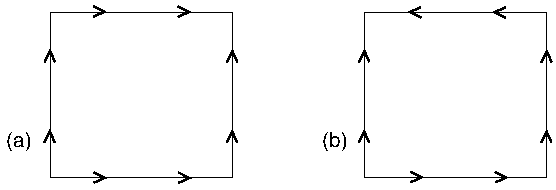
\includegraphics[width=0.78\linewidth]{figures/fig_8_6.pdf}
\caption{(a) トーラスと (b) Klein の壺を定義する同一視。}
\label{fig:8.6}
\end{figure}

また、オリエンティフォールド固定平面から離れた場所では、局所的な物理は\textbf{向きのある}弦理論のものであることにも注意しよう。元の向きのない理論では、射影は局所的に状態の半分を取り除くが、ここでは式 (8.8.3) のように、任意の点での弦の波動関数を、その像の点での値に関係付ける。

オービフォールド構成とオリエンティフォールド構成の相違の一つは、後者にはツイスト状態に直接対応するものがないことである。Klein の壺には、モジュラー変換 $\tau\to-1/\tau$ がないからである。トーラスと Klein の壺を示した図8.6を考えよう。トーラスでは、射影演算子は図8.6(a)の時間方向にツイストを挿入する。図を $90^\circ$ 回転すると、これは空間方向のツイストとなり、スペクトルにツイスト状態が存在することを意味する。しかし図8.6(b)の Klein の壺を $90^\circ$ 回転すると、向かい合う二つの辺で時間の向きが一致せず、このチャネルを中間状態によって解釈することはできない。したがって、オリエンティフォールド平面は力学的になりえないことに注意すべきである。D ブレーンの場合とは異なり、オリエンティフォールド平面に結び付いて、その形状の揺らぎを表す弦のモードはない。重力波が D ブレーンを振動させるという直観的な議論は、オリエンティフォールド平面には適用できない。本質的には、同一視 (8.8.3) が固定平面での境界条件となり、入射波と反射波が打ち消し合う。D ブレーンの場合、反射波は弦結合に関して高次である。

向きのある弦は、その向きを示す矢印を付けて描く。向きのない理論では、矢印を省いてもよいし、二つの向きの線形結合を取ってもよい。後者の描像は離散対称性をゲージ化する考え方とよりよく合致し、また、より一般的である。オリエンティフォールドではパリティ操作に時空変換が伴うので、単に矢印を忘れることはできない。

オリエンティフォールド構成は T 双対性を通して導入したが、トーラスコンパクト化の単なる T 双対ではない、より一般のオリエンティフォールドも考えられる。その場合は、世界面パリティとさまざまな時空対称性を組み合わせた群をゲージ化する。

\begin{figure}[tbp]
\centering
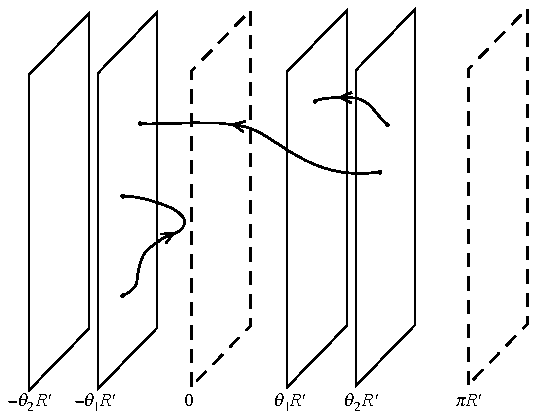
\includegraphics[width=0.78\linewidth]{figures/fig_8_7.pdf}
\caption{$0$ と $\pi R'$ にあるオリエンティフォールド平面、$\theta_1R'$ と $\theta_2R'$ にある D ブレーン、および $-\theta_1R'$ と $-\theta_2R'$ にある D ブレーンの像。ツイスト演算子 $\Omega$ は、時空反射と向きの矢印の反転を組み合わせて、任意の弦に作用する。したがって、2から1の像へ向かう弦は、1から2の像へ向かう弦になる。}
\label{fig:8.7}
\end{figure}

\subsubsectionlink*{開弦}

開弦の場合も状況は同様である。便宜上、一つのコンパクト方向に注目しよう。やはり、一方のオリエンティフォールド固定平面は0に、もう一方は $\pi R'$ にある。$SO(n)$ の Chan--Paton 因子を導入すると、一般の Wilson 線は対角形にできる。シンプレクティック群の場合も同様に進む。$n$ が偶数なら、固有値は対になり、
\begin{equation}
W=\operatorname{diag}
\left(e^{i\theta_1},e^{-i\theta_1},
e^{i\theta_2},e^{-i\theta_2},\ldots,
e^{i\theta_{n/2}},e^{-i\theta_{n/2}}\right)
\tag{8.8.4}\label{eq:8.8.4}
\end{equation}
となる。したがって双対な描像では、線分 $0\leq X'^{25}\leq\pi R'$ 上に $n/2$ 枚の D ブレーンがあり、オリエンティフォールド同一視によるそれらの像の点にも $n/2$ 枚ある。図8.7のように、D ブレーンとその像の間にも弦を張れる。一般のゲージ群は $U(1)^{n/2}$ である。向きのある場合と同様、$r$ 枚の D ブレーンが一致すると $U(r)$ ゲージ群が現れる。しかし今度は、その $r$ 枚の D ブレーンがさらに固定平面の一つにあると、これらのブレーンの一つと像のブレーンの一つを結ぶ弦も質量を失い、$SO(2r)$ を完成させるのにちょうど必要な追加状態のスペクトルが得られる。すべてのブレーンが一つのオリエンティフォールド平面上で一致すると、最大の $SO(n)$ が回復する。この最大対称性の場合が、二つの固定平面の間では非対称であることに注意しよう。

$n$ が奇数なら、$W$ の最後の固有値は $\pm1$ なので、T 双対な描像では、いずれか一方のオリエンティフォールド平面上に固定される。像をもたないため、例えば質量で測れば、これは実際には半分の D ブレーンである。また、$n=2$ で Wilson 線 $\operatorname{diag}(1,-1)$ を考えると、これは $O(2)$ には属するが $SO(2)$ には属さず、一枚の D ブレーンとその像の代わりに、各固定平面に一つずつ、二つの半 D ブレーンがある。

オリエンティフォールド平面は D ブレーンと同様に、ディラトンと計量に結合する。振幅は前節と同様だが、アニュラスが Klein の壺と Möbius 帯に置き換わる。実は、関係する計算は第7章ですでに行った。そこでは、$SO(2^{13})$ に対して全ディラトン結合が相殺されることを見いだした。T 双対な描像では、オリエンティフォールド平面の全ディラトン結合が、$2^{12}$ 枚の D ブレーンの結合を打ち消す。像は数えない。$k=25-p$ 個の方向で T 双対変換すると、固定平面は $2^k$ 個あり、その座標は0と $\pi R'_m$ のあらゆる組合せである。したがって、一つの固定平面の有効作用は
\begin{equation}
2^{12-k}T_p\int d^{p+1}\xi\,
e^{-\Phi}(-\det G_{ab})^{1/2}
\tag{8.8.5}\label{eq:8.8.5}
\end{equation}
であり、積分はその固定平面上で行う。

オリエンティフォールドにはツイストセクターに直接対応するものはないが、ある意味では開弦こそがツイスト状態であると論じられてきた。ここではこの点を強調しないことにする。類推が完全ではないからである。$\Omega$ のゲージ化自体は世界面に境界を導入しない。しかし、ディラトンのタドポールを相殺するために、オリエンティフォールド理論へ開弦を加えるのが自然であるという、明確な物理的意味はある。この相殺は、超弦において重要な役割を果たす。

\subsectionlink*{演習問題}
\addcontentsline{toc}{subsection}{演習問題}

\subsubsection*{演習8.1}\label{ex:8.1}
(a) 等時刻交換関係 (8.2.21) を導け。

(b) (8.2.22) の形の頂点演算子が、同時刻で有限の距離だけ離れているときに可換であることを、計算の詳細を示して確認せよ。

\subsubsection*{演習8.2}\label{ex:8.2}
周期方向が一つの場合に、巻き付き数が $+1,-1,0,0$、コンパクト方向の運動量がすべてゼロの、四つの閉弦タキオンの散乱振幅を計算せよ。

\subsubsection*{演習8.3}\label{ex:8.3}
時空に依存しない背景について T 双対性を示した。変化する計量 $G_{25,25}(x^\mu)$ をもつ背景は、逆計量 $G_{25,25}(x^\mu)^{-1}$ をもつ背景と T 双対であると予想される。原理的には、静的な配置のまわりで展開して示せるが、次のように直接示すことも有用である。

(a) 背景が $X^{25}$ の並進に対して不変であることだけを要求し、一般の質量のない背景中を動く弦の世界面作用を書け。座標 $X^{25}$ の周期を $R$ とする。

(b) $\partial_aX^{25}$ を $\partial_aX^{25}+A_a$ に置き換えると、$X^{25}$ の並進が世界面上の局所対称性になることを示せ。

(c) 世界面作用に $i\phi F_{ab}$ の項を加えよ。ここで $\phi(\sigma)$ は新しい場、$F_{ab}$ は $A_a$ の場の強さである。$\phi$ の経路積分は場の強さをゼロに強制するので、ゲージ場は自明になる。これは実質的に、段階 (b) を元に戻す。ゲージ $\partial_aA^a=0$ では、得られる理論が元の理論を書き直しただけであることを論じよ。

(d) ゲージ $X^{25}=0$ に到達できることを示し、次に $A_a$ について Gauss 型経路積分を行え。古典的に扱い、行列式は無視せよ。$\phi$ を $X'^{25}$ に適切な定数を掛けたものと同一視すると、得られる作用が、T 双対理論に期待される形をもつことを示せ。ディラトンの変換 (8.3.31) を得るには、$A_a$ の経路積分を1ループまで行う必要がある。また、$X'^{25}$ の座標周期を得るには、やや注意深い議論が必要である。（参考文献：Buscher (1987, 1988)\cite{Buscher:1987sk,Buscher:1987qj}、Roček \& Verlinde (1992)\cite{Rocek:1991ps}。）

\subsubsection*{演習8.4}\label{ex:8.4}
複数のコンパクト方向について、直接計算した弦の分配関数と、経路積分で計算したものが等しいことを確認せよ。式 (8.4.12) の下のコメントを参照せよ。

\subsubsection*{演習8.5}\label{ex:8.5}
(a) コンパクト方向が一つの場合のスペクトル (8.4.26) が、偶自己双対格子を定義することを示せ。

(b) スペクトル (8.4.7) について同じことを行え。

\subsubsection*{演習8.6}\label{ex:8.6}
第8.4節の、周期方向が二つの場合の例において、一般の運動項 (8.4.35) が (8.4.39) の形に帰着することを示せ。$\tau$ と $\rho$ が両方とも純虚数である特別な場合に、さまざまな双対性の $\tau$ と $\rho$ への作用についての主張を確認せよ。

\subsubsection*{演習8.7}\label{ex:8.7}
(a) D$p$ ブレーン上の波の散乱振幅を計算せよ。すなわち、四つの集団座標の頂点演算子を含む木レベル振幅を考えよ。偏極がすべての運動量に直交することに注意せよ。これにより大きく簡単になる。

(b) Regge 極限と硬散乱極限を調べよ。

(c) 低運動量極限を取り、作用 (8.7.2) から得られるものと比較せよ。

\subsubsection*{演習8.8}\label{ex:8.8}
一致する二枚の D$p$ ブレーンについて、前問を繰り返せ。今度は集団座標が Chan--Paton 因子を含む。特に (c) の変化に注目せよ。

\subsubsection*{演習8.9}\label{ex:8.9}
(a) $p+1$ 個の座標に Neumann 境界条件、$25-p$ 個の座標に Dirichlet 境界条件を課し、円板内部にある $n$ 個の指数型頂点演算子の期待値を計算せよ。

(b) 内部の演算子 $\partial_aX^M$ も含むように計算を拡張せよ。

\subsubsection*{演習8.10}\label{ex:8.10}
前問の結果から、D$p$ ブレーンが重力子を放出する振幅を計算せよ。D$p$ ブレーンの有効作用、および結合に関する結果 (8.7.28) と比較せよ。

\subsubsection*{演習8.11}\label{ex:8.11}
(a) 演習8.9の境界条件に対して、二つの閉弦タキオンを含む円板振幅を計算せよ。これは D ブレーンによる閉弦の散乱に対応する。

(b) Regge 極限と硬散乱極限を調べよ。

(c) 振幅が中間の開弦に由来する極をもつことを示せ。物理的解釈を与えよ。

\subsubsection*{演習8.12}\label{ex:8.12}
(a) 前問の計算を、より煩雑だが、より興味深い、質量のない閉弦の場合に行え。

(b) 重力子振幅に、開弦の集団座標による極があることを示し、作用 (8.7.2) を用いた計算と比較せよ。

(c) 反対称テンソルと開弦の光子について同じことを行え。
